\section{Results III: a registered failure, diagnosed and repaired inside the framework}
\label{sec:arc}

This section is the paper's centerpiece, and Figure~\ref{fig:cycle} is its map: a registered failure (E2), a diagnosis using the framework's own exact-input machinery, a corrected statistic re-registered with a \emph{predicted failure to beat the baseline} among its frozen predictions (E7), and two generalizations---to circuit-level noise (E8) and to closed-loop decoder control (E9). Throughout, E2's committed verdicts stand untouched; everything here is additive.

\begin{figure}[htbp]
\centering
\begin{tikzpicture}[
  x=1in, y=1in, font=\small,
  stage/.style={rounded corners=3pt, line width=0.6pt,
    align=center, inner sep=4pt, outer sep=0pt, minimum height=1.70in},
  substage/.style={rounded corners=3pt, line width=0.6pt,
    draw=black!50, fill=black!4, font=\footnotesize,
    align=center, inner sep=3pt, outer sep=0pt, text width=1.52in},
  flow/.style={-{Stealth[length=5pt,width=5pt]}, line width=0.8pt}
]
% A 6.5in by 4.6in canvas includes the legend and balanced outer margins.
\path[use as bounding box] (0,0) rectangle (\linewidth,4.60in);

% Top row: equal-height boxes and two 0.45in horizontal connectors.
\node[stage, draw=red!60!black, fill=red!8,
  text width=\dimexpr1.80in-8pt\relax] (s1) at (1.00,3.65)
  {E2: registered prediction P2.1 fails as frozen};
\node[stage, draw=blue!60!black, fill=blue!8,
  text width=\dimexpr1.85in-8pt\relax] (s2) at (3.275,3.65)
  {Exact-input diagnosis with the framework's own machinery: Walsh--Hadamard pmf inversion, $A^{*}$-lift energy compression, mis-scaled null};
\node[stage, draw=blue!60!black, fill=blue!8,
  text width=\dimexpr1.75in-8pt\relax] (s3) at (5.525,3.65)
  {Corrected statistic re-registered, including a prediction that the original scenario will \textsc{still} not beat the baseline};

% Bottom-left stage: one container with a heading and two internal boxes.
\node[stage, draw=black!50, fill=black!4, minimum width=1.80in]
  (s5) at (1.00,1.25) {};
\node[font=\small\bfseries, inner sep=0pt] at (1.00,1.92)
  {Generalization};
\node[substage, minimum height=0.68in] (e8) at (1.00,1.45)
  {E8: circuit level (Stim, $d{=}3$); $2\times$ bar met at the grid's thinnest margin};
\node[substage, minimum height=0.53in] (e9) at (1.00,0.775)
  {E9: closed recalibration loop on a known drifting channel};

% Bottom-right stage: one rounded outline, equal halves, one divider.
\begin{scope}
  \clip[rounded corners=3pt] (2.35,0.40) rectangle (6.40,2.10);
  \fill[green!10] (2.35,0.40) rectangle (4.375,2.10);
  \fill[orange!12] (4.375,0.40) rectangle (6.40,2.10);
\end{scope}
\draw[green!50!black, line width=0.6pt, rounded corners=3pt]
  (4.375,0.40) -- (2.35,0.40) -- (2.35,2.10) -- (4.375,2.10);
\draw[orange!70!black, line width=0.6pt, rounded corners=3pt]
  (4.375,2.10) -- (6.40,2.10) -- (6.40,0.40) -- (4.375,0.40);
\draw[black!50, line width=0.6pt] (4.375,0.40) -- (4.375,2.10);
\node[align=center, inner sep=4pt,
  text width=\dimexpr2.025in-8pt\relax] at (3.3625,1.25)
  {E7 off-support $(4,8)$: W2b at full detection by $N{=}1000$; neither baseline meets the criterion within the grid};
\node[align=center, inner sep=4pt,
  text width=\dimexpr2.025in-8pt\relax] at (5.3875,1.25)
  {E7 original $(0,3)$: predicted failure to beat the baseline held (baseline 1000 vs.\ corrected 4000)};
\coordinate (s4north) at (5.525,2.10);
\coordinate (s4west) at (2.35,1.25);

% The only arrows are the five straight edges of the clockwise loop.
\draw[flow] (s1.east) -- (s2.west);
\draw[flow] (s2.east) -- (s3.west);
\draw[flow] (s3.south) -- (s4north);
\draw[flow] (s4west) -- (s5.east);
\draw[flow, line width=1.4pt] (s5.north) -- (s1.south);

\node[font=\small, align=center, text width=3.10in, inner sep=0pt]
  (thesis) at (3.25,2.45)
  {\textbf{the framework audits and repairs\\its own instrument}};

\node[font=\footnotesize, align=center, text width=6.30in, inner sep=0pt]
  at (3.25,0.175)
  {red = registered failure; blue = framework-internal diagnosis and re-registration; green = registered positive; amber = predicted negative that held};
\end{tikzpicture}

\caption{The diagnosis-and-repair cycle of this section. A registered failure (E2, red) is diagnosed with the framework's own exact-input machinery (blue); the corrected statistic is re-registered together with a prediction that the original scenario will \emph{still} not beat the baseline (blue); the predicted negative holds while the off-support scenario detects (amber / green); and the correction generalizes to circuit level (E8) and to a closed loop (E9). The label inside the loop states the arc's thesis: the framework audits and repairs its own instrument.}% C-03
\label{fig:cycle}
\end{figure}

\subsection{The failure (E2)}
\label{sec:e2}

E2 tested drift detection on SURF(3): declared model N2 ($p = 3/100$), true model N3 (the same plus an unmodeled correlated $ZZ$ injection, $q = 1/50$, on the frozen qubit pair $(0,3)$). Two witnesses were tested against a matched decoder-failure-rate baseline: W1, an \emph{oracle} witness with simulator access to true logical values (labeled non-deployable from the start), and W2, the deployable-shaped, syndrome-only witness---the one that would matter in practice. Results (\gMeasured): W1 detected at $N = 500$ shots vs.\ the baseline's $1000$---a real $2\times$ improvement, short of the registered $4\times$ bar---and W2 \emph{never detected within the frozen grid} (up to $N = 16000$). Both registered predictions failed (\gRegNeg). % F-026, F-005 (C-24)
Null calibration passed: false-positive rates 0.0 (W1) and 0.02 (W2) at the frozen bar. % F-027

\subsection{The diagnosis: exact inputs, and mostly about the test itself}
\label{sec:diagnosis}

Before any correction code was written, the failure was analyzed with the same moment engine the audits are built on: the mean shifts, covariance blocks, and syndrome distributions below are exact rational objects, and the scalar energies and divergences reported from them are floating-point evaluations of those exact inputs. The four findings were then pinned as tests in the repository, so they are commitments, not narrative. The reflexive point we draw from findings 1 and 2 is an analogy, marked as such (\gInterp): the same moment machinery that audits a schedule's coverage of the logicals was turned on the witness itself, to ask how much of the drift signal it kept.

\paragraph{Finding 1: the statistic discards its mean signal (\gExact).} W2 was built from \emph{centered} covariance blocks, so the drift's direct first-moment signal entered it only through its second-order footprint, never as a mean feature. The frozen injection's exact mean shift is zero on seven of eight native checks and $-331776/9765625 \approx -0.0340$ on the eighth, with total energy $\|\Delta\mathrm{mean}_L\|^{2} = 0.0011542$, a floating-point sum of the exact entries. % F-075 (C-25)
A real, exactly quantified direct signal was being left out of the feature set.

\paragraph{Finding 2: the lift built for the wrong objective compresses the signal $\approx 73\times$.} W2 lifted the syndrome-covariance defect through the coverage-optimal map $A^{*}$---a map fit to predict \emph{logical values}, not to preserve \emph{drift sensitivity}. The drift signal's energy before the lift is $\|\Delta K_{LL}\|_F^{2} = 0.0032632$; after, $4.4703 \times 10^{-5}$ (floating-point norms of exact covariance differences). % F-076 (C-26)
The compression ratio $\approx 73\times$ is our reading of those two numbers (\gInterp).

\paragraph{Finding 3: a borrowed null (\gInterp, confirmed by measurement below).} W2's alarm threshold was calibrated on W1's statistic---a differently scaled object---rather than on W2's own null distribution. % F-077 (C-27)

\paragraph{Finding 4: the frozen scenario is structurally hard for \emph{any} syndrome-only method.} The key move: because means of XOR-combinations of checks are Walsh--Hadamard coefficients of the syndrome distribution (Section~\ref{sec:domain}), the full $2^{8}$-outcome native-check syndrome pmf is \emph{exactly} recoverable under both the declared and true models, hence so is the syndrome distribution under both models (\gExact). From those exact distributions, the per-shot Kullback--Leibler divergence $D(\mathrm{true}\,\|\,\mathrm{declared})$ of the syndrome channel, in nats per shot, is evaluated numerically; by Stein's lemma it is the exponential rate at which i.i.d.\ samples discriminate the two hypotheses~\cite{cover2006elements}. We compare it with the per-shot divergence of the logical-failure channel, measured from $N = 2 \times 10^{6}$ shots per scenario (\gMeasured), over three injection pairs: % F-078 (C-28a, C-28b)

\begin{table}[htbp]
\centering\footnotesize
\setlength{\tabcolsep}{3.5pt}
\begin{tabular}{l l r r r}
\toprule
Pair & Relation to logical support & syndrome KL/shot & failure KL/shot & ratio \\
 & & (from exact pmf) & (measured) & \\
\midrule
$(0,3)$, the frozen E2 pair & 2 of 3 qubits of $\bar{Z}$ & 0.006151 & 0.009247 & 0.665 \\ % F-078
$(2,5)$ & 1 qubit touches $\bar{X}$ & 0.010823 & 0.009841 & 1.100 \\ % F-078
$(4,8)$ & off both logical supports & 0.051352 & 0.000066 & 773.4 \\ % F-078
\bottomrule
\end{tabular}
\caption{Per-shot KL divergence (nats/shot) available to the syndrome channel, evaluated from the exactly recovered pmf, vs.\ the logical-failure channel, measured; the ratio is therefore a measured quantity (\gMeasured). The frozen E2 pair $(0,3)$ sits, by construction, nearly on a minimum-weight logical-failure path: the failure channel carries more per-shot information about such drift than the syndrome does (ratio $< 1$), while for the off-support pair the syndrome channel carries $\approx 773\times$ more. Per-shot divergence is a discrimination rate, not a finite-sample latency ratio.} % F-078 (C-28a, C-28b)
\label{tab:kl}
\end{table}

The structural reading (\gInterp): drift that feeds a minimum-weight failure path is exactly the drift the failure channel is built to notice and the syndrome channel is built to correct silently. Among the three scenarios, the E2 pair is the one that puts a syndrome-only witness at the greatest disadvantage relative to failure-rate monitoring---a fact about this scenario grid, not a general worst-case statement---independent of, and in addition to, findings 1--3. This finding drove the design of the re-registration: the corrected witness had to be tested across the \emph{range} finding 4 exposes, with an honest prediction attached to each regime.

\subsection{The corrected witness, re-registered---including a predicted failure (E7)}
\label{sec:e7}

The correction unifies findings 1 and 2 in one object: the vector of means of the degree-$\le 2$ probe family (all 8 native checks plus all 28 pairwise XOR products---36 exact Walsh--Hadamard coefficients), used \emph{directly}, with no centering and no lift. The corrected detection statistic is the whitened quadratic form (a model-referenced Mahalanobis form of Hotelling type~\cite{hotelling1931ratio}; unlike the classical $T^{2}$, the covariance is the declared model's, not a sample estimate)
\begin{equation}
T \;=\; (\hat\theta - \theta_{\mathrm{model}})^{\top}\, \Sigma_{\theta}^{+}\, (\hat\theta - \theta_{\mathrm{model}}),
\label{eq:w2b}
\end{equation}
with $\theta_{\mathrm{model}}$ and the estimator covariance $\Sigma_\theta$ exact under the declared model and the threshold calibrated on the statistic's own null by seeded parametric bootstrap (Monte Carlo draws from the declared model)~\cite{efron1979bootstrap}. Around it, a ladder of four rungs was registered: the \emph{old} statistic with its null merely recalibrated (isolating finding 3); the quadratic statistic of Eq.~\eqref{eq:w2b}; a matched-filter \emph{naming} step (a dictionary of nine exact per-qubit drift signatures, whitened, inner-product-matched, then forward-mapped to a logical direction); and a CUSUM sequential wrapper~\cite{page1954continuous}---with the baseline given the \emph{same} sequential upgrade, which removes one test-design asymmetry between the two sides (it does not equalize their operating characteristics; the null-rate checks below report those separately). Seven predictions were frozen from finding 4's numbers before implementation. Three outcomes carry the section (Figure~\ref{fig:e7}):

\paragraph{The off-support scenario: a dramatic, registered win.} On pair $(4,8)$---where Table~\ref{tab:kl}'s measured ratio put $\approx 773\times$ more per-shot information in the syndrome channel---the corrected rungs detect at $N = 1000$ (quadratic and naming rungs) and $N = 2000$ (sequential), while neither baseline reaches the detection criterion ($\ge 9/10$ seeds) anywhere in the frozen grid up to $N = 16000$ (\gRegPos{} against a conservative registered $10\times$ bar). % F-078, F-080 (C-28b, C-30)

\paragraph{The original scenario: the predicted failure held.} We registered, in advance, backed by Table~\ref{tab:kl}'s ratio of $0.665$, that on the original E2 pair $(0,3)$ \emph{no corrected rung would beat the baseline}. That is what happened: baseline $N = 1000$; best corrected rungs $N = 4000$ (\gRegPos---a predicted negative that held). % F-081 (C-31)
We give this result more narrative weight than the win above, deliberately. A correction developed after a failure invites the suspicion of post-hoc storytelling---of a statistic quietly tuned until the old test passes, the degenerating move in Lakatos's sense~\cite{lakatos1978methodology}. A frozen, exact-computation-backed prediction that the correction would \emph{still lose} on the original test, which then held, is the strongest evidence this arc can offer that the diagnosis was explanatory rather than curve-fitting. The near-parity scenario $(2,5)$, registered as descriptive with no bar, landed where its ratio of $1.100$ suggested: baseline $1000$; quadratic and naming rungs $2000$; sequential rung $8000$ (\gMeasured). % F-082

\paragraph{The honest residue.} Three E7 predictions failed (\gRegNeg{} each). The recalibrated-null prediction P7.1 failed: we predicted the old statistic's own-null threshold would be $\le 10\%$ of the borrowed one, and measured a ratio of $1.33$. % F-079 (C-29)
The reading (\gInterp): our $O(p)$-vs-$O(p^2)$ reasoning had described the \emph{injected signal's} scale, not the \emph{null-fluctuation} scale a threshold actually calibrates.
Naming split (Figure~\ref{fig:naming}): only 3/10 detecting seeds named a qubit in the true injection pair (bar: 8/10), while the forward-mapped logical-direction overlap was $0.869$, above its $0.6$ bar (\gMeasured). % F-083 (C-32)
The reading (\gInterp): the overlap is taken in the two-dimensional space of the selected logical observables, onto which the nine per-qubit drift signatures map to few distinct directions, so direction overlap is a coarse check that detection and direction-naming can pass while qubit-level naming stays hard. The headline quadratic rung W2b's null false-positive rate came in at 6\% against the 2\% bar (all other rungs passed). % F-084 (C-32)

\begin{figure}[htbp]
\centering
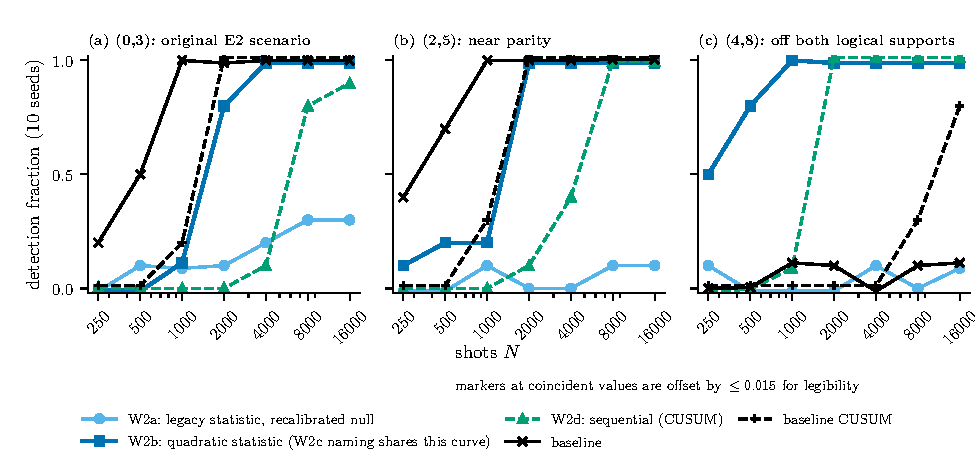
\includegraphics{figures/generated/fig_F6_e7_detection_ladder.pdf}
\caption{Corrected-witness detection fraction versus shots across the E7 scenario grid, 10 seeds per point (\gMeasured). (a) The original E2 pair $(0,3)$: the baseline detects first, which was the registered, expected outcome, not a surprise (P7.3; \gRegPos{} as a predicted negative that held). (b) The near-parity pair $(2,5)$, registered as descriptive with no bar. (c) The off-support pair $(4,8)$: the quadratic statistic W2b (whose detection curve the naming rung W2c shares) reaches full detection at $N = 1000$ while neither baseline reaches the $\ge 9/10$ detection criterion anywhere in the grid; W2a is the legacy statistic with only its null recalibrated (\gRegPos{} against a registered $10\times$ bar).}% F-080, F-081, F-082 (C-30, C-31)
\label{fig:e7}
\end{figure}

\begin{figure}[htbp]
\centering
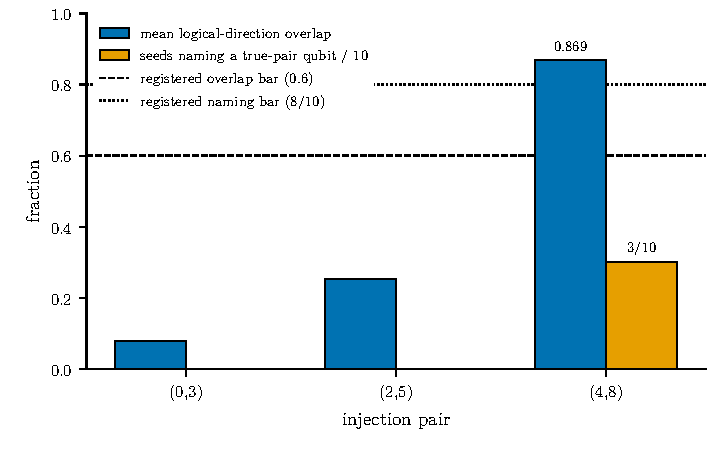
\includegraphics{figures/generated/fig_F7_e7_naming_overlap.pdf}
\caption{The E7 naming outcome (P7.5; \gRegNeg). On the off-support pair $(4,8)$ the forward-mapped logical-direction overlap is $0.869$, above the registered $0.6$ bar, while only 3 of 10 detecting seeds named a qubit in the true injection pair, below the $8/10$ bar. Pairs $(0,3)$ and $(2,5)$ are shown for context; the prediction concerned $(4,8)$. The reading (\gInterp): the overlap is taken in the two-dimensional space of the selected logical observables, onto which the nine per-qubit signatures map to few distinct directions, so it is a coarse check that cannot discriminate between qubits on its own.}% F-083 (C-32)
\label{fig:naming}
\end{figure}

\subsection{Generalization to circuit-level noise (E8)}
\label{sec:e8}

The corrected statistic generalizes directly to circuit level: detectors replace checks, the degree-$\le 2$ family becomes detectors plus pairwise XOR products (40 detectors, 820 features for the rotated $d{=}3$ Stim memory circuit used), % F-088
and---because the prototype has no exact moment engine at circuit level---$\theta_{\mathrm{model}}$ and $\Sigma_\theta$ are estimated from a large declared-model calibration sample ($2 \times 10^{5}$ shots), with predictions frozen from a disjoint-seed pilot before the scored run (Section~\ref{sec:methods-registration}). % F-089
The scored drift scenario is a global $2\times$ error-rate increase; the baseline is the PyMatching logical-failure rate under the same detection framing.

Result (Figure~\ref{fig:e8}): the witness detects at $N_{\mathrm{det}} = 50$ vs.\ the baseline's $100$, clearing the pilot-frozen $2\times$ bar exactly---which, on the discrete grid $\{10, 20, 50, 100, 250, 500, 1000, 2000\}$, is the thinnest margin the grid can resolve, and this result must be read with that caveat attached, not as a comfortable win (\gRegPos, margin caveat mandatory). % F-086 (C-33)
Null false-positive rates were 0\% for both sides (\gRegPos). % F-087
We report one more thing the deviations log preserves: the pilot had suggested $\approx 5\times$; the scored run delivered $2\times$. The pilot number is a smaller-sample estimate and is not the headline. % F-167, F-086

\begin{figure}[htbp]
\centering
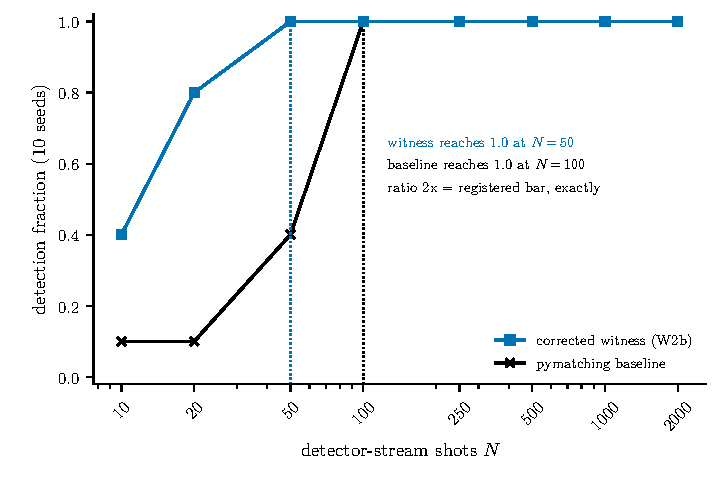
\includegraphics{figures/generated/fig_F8_e8_circuit_level.pdf}
\caption{Circuit-level detection fractions under a global $2\times$ rate drift on the rotated $d{=}3$ Stim memory circuit, 10 seeds (E8; \gRegPos). The corrected witness reaches full detection at $N_{\mathrm{det}} = 50$ and the PyMatching baseline at $100$: the witness clears the pilot-frozen $2\times$ bar exactly, at the thinnest margin this discrete grid can resolve, and not by a comfortable margin.}% F-086, F-088 (C-33)
\label{fig:e8}
\end{figure}

\subsection{Closing the loop: witness-triggered decoder recalibration (E9)}
\label{sec:e9}

The final experiment asks whether the witness's information is worth anything \emph{operationally}: does the witness's \emph{timing} buy logical fidelity per unit of recalibration budget, when the drifting channel is known by construction and only \emph{when} to recalibrate is at issue? On an epoch-discretized circuit-level timeline (72 detectors, 2628 degree-$\le 2$ features) % F-090
with a heterogeneous drift injected partway through (one measurement-flip channel elevated $20\times$---a uniform global rescale was verified, before freezing anything, to give minimum-weight matching nothing to recalibrate, and the scenario was corrected and logged), five decoder policies run over 10 seeds: \emph{static} (never recalibrate; floor), \emph{oracle} (switch to the true-model decoder at the true drift epoch, without charging a recalibration event; ceiling), \emph{budget-matched blind schedule}, \emph{high-budget blind schedule} ($\approx 5\times$ the events), and the \emph{witness-triggered} policy (recalibrate when the sequential witness fires, self-correcting on false alarms).

The budget matching deserves one sentence of methodology, because it is where an experiment like this is easiest to rig accidentally: the matched schedule was forced, per seed, to spend \emph{exactly} the same number of recalibration events the witness policy spent on that seed (realized counts $[1,1,2,2,1,1,3,2,1,2]$, identical lists for both policies; mean 1.6), % F-093
after the first frozen run was caught in internal review: its schedule had been set to a fixed period aimed at one event per run while the witness policy's realized mean was $1.6$, so the budgets were not matched even in aggregate. The schedule was corrected to exact per-seed matching and the implementation re-run and re-frozen, with the prediction bars unchanged (Appendix~\ref{app:deviations}).

Results (Figure~\ref{fig:e9}; post-drift logical error rate per epoch, mean over seeds; grade per item):
\begin{itemize}
\item Witness-triggered: $0.0930$, about $0.0014$ above the oracle ceiling's $0.0916$ (gap $0.00143$ to three significant figures; frozen bar: within $0.01$; \gRegPos). % F-091 (C-34; rounding authorized in claims.md)
\item Against the genuinely budget-matched blind schedule: $0.0930$ vs.\ $0.1115$---the witness wins by $0.0185$ at \emph{identical} per-seed budgets (\gRegPos). % F-092, F-093 (C-34)
\item The static floor sits at $0.1185$. % F-097
\item The high-budget schedule ($\approx 5\times$ the events) scores $0.0946$, and its $0.0016$ deficit to the witness policy is smaller than the $\approx 0.002$ estimated paired standard error at 10 seeds---statistically unresolved, and we state so in the same breath as the number (\gMeasured, no bar). % F-094, F-095 (C-35)
\item Pre-drift trigger rates, descriptive: witness 0.0 on the scored seeds; the schedules trigger by construction (0.5 and 1.0 of seeds recalibrating pre-drift at least once). % F-096
\end{itemize}

Two scope statements bound this result. First, the resolved claim is \emph{witness beats budget-matched blind scheduling}; whether it beats \emph{frequent} blind scheduling is unresolved at this sample size---spending $\approx 5\times$ the budget blindly closes most, not all, of the gap. % C-35
Second, E9's recalibration deliberately searches only the one channel known by construction to drift: it demonstrates the \emph{timing and budget} value of the witness, not drift \emph{identification}, which is E7's naming step, tested separately. % C-39 (F-105)

\begin{figure}[htbp]
\centering
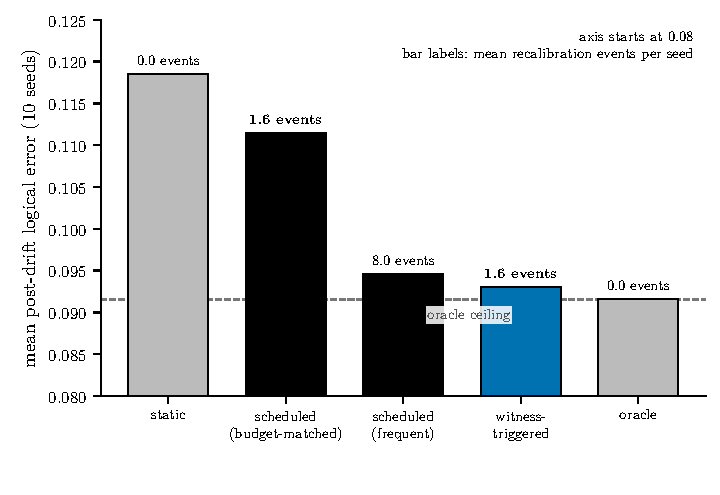
\includegraphics{figures/generated/fig_F9_e9_closed_loop.pdf}
\caption{Closed-loop decoder recalibration (E9): mean post-drift logical error per epoch over 10 seeds, with each policy's mean recalibration events per seed above its bar (\gMeasured). Recalibration here re-estimates the one channel known by construction to drift; the oracle switches to the true-model decoder at the drift epoch without spending a recalibration event, which is why it shows $0.0$ events. The witness-triggered policy and the budget-matched blind schedule spend identical realized event counts on every seed (counts between 1 and 3, mean $1.6$), and the witness wins by $0.0185$ (\gRegPos). The frequent schedule spends about $5\times$ the budget; its $0.0016$ deficit to the witness is smaller than the $\approx 0.002$ paired standard error at 10 seeds and is statistically unresolved, so this figure does not show that the witness beats frequent blind recalibration.}% F-091, F-092, F-093, F-094, F-095 (C-34, C-35)
\label{fig:e9}
\end{figure}

% ===========================================================================
